\documentclass{article}

\usepackage[english]{babel}
\usepackage[letterpaper,top=2cm,bottom=2cm,left=3cm,right=3cm,marginparwidth=1.75cm]{geometry}

\usepackage{amsmath}
\usepackage{graphicx}
\usepackage[colorlinks=true, allcolors=blue]{hyperref}

\title{Data mining: Assignment 3}
\author{Arno Deceuninck}

\begin{document}
\maketitle

\section{Word embeddings}
In order to find clusters in the data (and thus also determine the number of clusters), we need to transform the given sentences (from the articles) into vectors, so we can run some known algorithms on it. I first tried to do this by using TfIdf (which generates a sparse vector based on the term frequency and the inverse document frequency). This didn't really give clear clusters, so I tried to get more of the semantic meaning of the paragraphs by using sentence-transformers. More specifically, I used the pre-trained all-MiniLM-L6-v2 model, since this is a general model recommended for many use cases that still performs quite good.

In order to visualize our clusters better, I used TSNE to map the high dimensional vectors from the TfIdfVectorizer or sentence-transformer to 2D space where a higher distance between two vectors in the higher dimensional space, would also result in a higher distance in the 2D space. A visualization for the TfIdf vectors can be found in figure \ref{fig:tsnetfidf} and for the sentence-transformers vectors in figure \ref{fig:tsnettransf}. Note that in the visualization, some points might apear quite far from other points in the clusters. This is because the clustering is maade in the higher dimensional space, while the visualisation only has two dimensions.


\begin{figure}[h!]
\centering
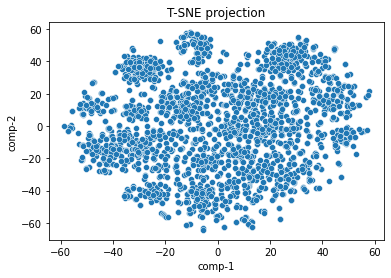
\includegraphics[width=75mm]{tsne-tfidf.png}
\caption{TSNE representation of the data (TfIdf)}
\label{fig:tsnetfidf}
\end{figure}

\begin{figure}[h!]
\centering
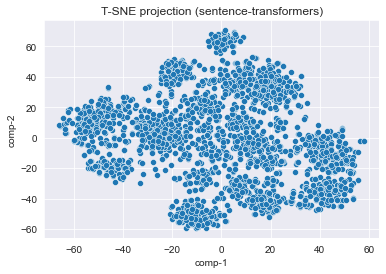
\includegraphics[width=75mm]{tsne-transformers.png}
\caption{TSNE representation of the data (sentence-transformers)}
\label{fig:tsnettransf}
\end{figure}

\section{Number of clusters}
There are two main methods for determing the number of clusters. We can either try running K-Means multiple times on a different number of clusters or we can run DBSCAN on it.

I started by trying to determine the number of clusters by running clusters of different sizes and plotting their SSE. If we reached the optimal number of clusters, the SSE would still decrease, but the decrease would be less outspoken. You can see this plot for the TfIdf embedding in figure \ref{fig:ssetfidf}. There isn't a clear elbow in this graph, only a slight kink somewhere between 11 and 23 clusters. In the SSE graph for the sentence-transformers (figure \ref{fig:ssetran}) the kink is still vague and still somewhere between 12 and 23 clusters, mainly around 13 clusters.

\begin{figure}[h!]
\centering
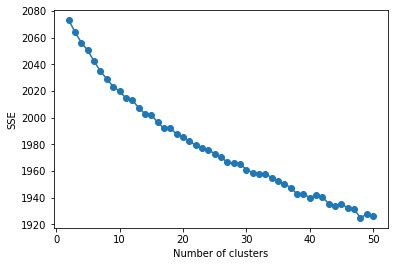
\includegraphics[width=75mm]{sse-tfidf.png}
\caption{SSE (TfIdf)}
\label{fig:ssetfidf}
\end{figure}


\begin{figure}[h!]
\centering
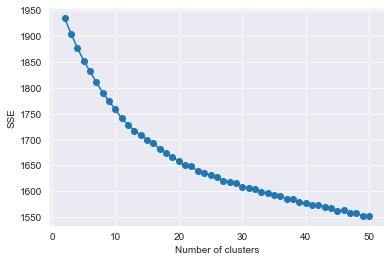
\includegraphics[width=75mm]{sse-transformers.png}
\caption{SSE (sentence-transformers)}
\label{fig:ssetran}
\end{figure}

Another pproach we can take is finding density-based clusters using DBSCAN. The advantage of this is that we don't need to know the number of clusters beforehand. The problem however is that there are two important parameters we need to specify, namely eps and min\_samples. To determine those parameters, I performed a grid search over those parameters and looked at the number of clusters they each gave. This gave some indications on where the eps and min\_samples parameters should be located, but when ploting those, you could see that they consisted of one huge cluster and a few smaller ones around them, so no useful data. Also plotting the number of clusters for a fixed epsilon and a variable minimum number of samples, didn't give better information on the amount of clusters.

Since the most signifant kink was at 13 clusters, I'll try to continue with that value and take a more detailed look at the clusters generated from this (to further improve the number of clusters estimation). A better answer and how confident I'm about this will come after the next section.

\section{Clustering methods}

KMeans won't always converge to the same solutions, which might cause some sub optimal solutions. It might have some problems when clusters have a different size or density, but that isn't really the case if we look at the TSNE plot. At first sight, the data also doesn't contain extreme outloiers, so this might give a good solution. Bisecting K-Means also seems suitable for this task. The density of our clusters is the same and they're of similar size, which make it suitable for KMeans.

In DBSCAN, we still need to determine the specified number of points (MinPts) and epsilon. There aren't clear borders between our clusters and there are a lot of noise points, so this method doesn't seem suitable. DBSCAN is quite resistant to noise and can handle clusters of different shapes and sizes, but in our scenario, it sees mainly one large cluster and a few smaller ones. Besides this, we're also working with high-dimensional data, for which DBSCAN does not work well. We don't really have varying densities in our data, so it's not a problem that DBSCAN doesn't work well with varying densities, but because of the other reasons, DBSCAN isn't suitable for us.

Finlly, we've also seen expectation maximization during the lectures. This isn't relevant for this clustering scenario, since we don't know the process that generated the clusters (i.e. it's manually generated by users and not using a model of which we can determine the parameters).

Hierarchical clustering would also have been an option with this data (since e.g. cryptography can be seen as a subcluster of mathematic or computer science), but in order to do this, we first have to generate the clusters and then merge clusters based on the proximity matrix. This is also not relevant for this assignment, since we're asked to only output one cluster number per title.

\section{KMeans}
We'll thus use KMeans to generate our clusters. As mentioned earlier (based on our experiments with both KMeans and DBSCAN), we'll first try to find 13 clusters using KMeans. When printing a few titles per cluster, you can see a clear connection between things inside one clustered. I tried assigning a category to each of them, of which the results can be found in figure \ref{fig:clusters13}.

\begin{figure}[h!]
\centering
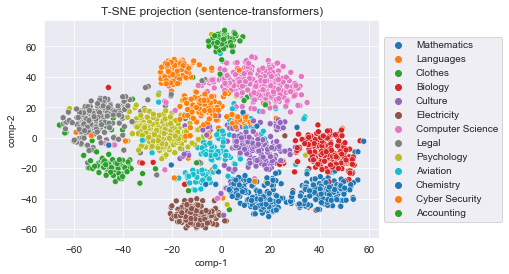
\includegraphics[width=150mm]{clusters-labeled-13.png}
\caption{Clusters (n=13, labeled with own interpretation)}
\label{fig:clusters13}
\end{figure}

This was the result for 13 clusters. Let's try to find more clusters and see whether the generated results still make sense. For 14 clusters, the languages and culture categories were split into three categories: 'Music \& Literature', 'Television' and 'Art'. This can be seen as a hierarchical clustering. The categories still make sense, so let's try to split it up even further. With 15 clusters, biology is split into biology and agriculture. This is still a split that makes sense. Note that the exact contents per cluster is stochastic. For more than 15 clusters, there start appearing categories that are too similar to each other and in which I can't find a clear correlation between the titles in the cluster, so my final guess for the number of clusters is 15 (you can find a visualization of the 15 clusters and my interpretation to each of them in figure  \ref{fig:clusters15}). I wasn't confident at all about the amount of clusters when I determined it in the 2nd section, since it had a wide range of possibilities. Now I've seen the articles per cluster, all 15 clusters make sense (which wasn't the case for 16 clusters), so I'm quite sure about this number.

\begin{figure}[h!]
\centering
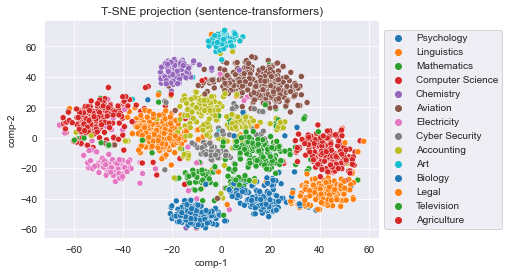
\includegraphics[width=150mm]{clusters-labeled-15.png}
\caption{Clusters (n=15, labeled with own interpretation)}
\label{fig:clusters15}
\end{figure}

\section{Code}
All used code can be found in 'assignment3.ipynb'. The data should be placed in the same directory as this notebook file and jupyter should also be run from this same folder.

\end{document}